\documentclass[a4paper,oneside,12pt]{article}
\usepackage[margin=0.7in]{geometry}
\usepackage{tikz}
\usepackage[cm-default]{fontspec}
\usepackage{xunicode}
\usepackage{xltxtra}
\usepackage{amsfonts}
\usepackage{amssymb}
\usepackage{amsmath}
\usepackage[utf8]{inputenc}
\usepackage[greek]{babel}
\usepackage{xgreek}
\usepackage{algpseudocode, listings}
\setmainfont[Mapping=tex-text]{CMU Serif}
\usepackage{titling}
\newcommand{\N}{\ensuremath{\mathbb N} }
\newcommand{\Z}{\ensuremath{\mathbb Z} }
\newcommand{\A}{\ensuremath{\mathcal A} }
\newcommand{\pset}[1]{\ensuremath{\mathcal P( #1 )}}
\newcommand{\pr}[1]{\ensuremath{\mathbb P [ #1 ]}}
\renewcommand{\vec}[1]{\ensuremath{\mathbf {  #1 }}}
\newcommand{\ev}[1]{\ensuremath{\mathbb E [ #1 ]}}
\newcommand{\R}{\ensuremath{\mathbb R}}
\DeclareMathOperator{\Ima}{Im}
\usepackage{float}

\newcommand*{\QEDA}{\hfill\ensuremath{\blacksquare}}
\newcommand*{\QEDB}{\hfill\ensuremath{\square}}
\usepackage[usenames,dvipsnames]{pstricks}
\usepackage{epsfig}
\usepackage{pst-grad} % For gradients
\usepackage{pst-plot}
\setlength{\droptitle}{-5em}
\usepackage{graphicx}

\makeatletter
\def\maxwidth{%
  \ifdim\Gin@nat@width>\linewidth
    \linewidth
  \else
    \Gin@nat@width
  \fi
}
\makeatother

\title{ \textbf{Νευρο-Ασαφής Έλεγχος \& Εφαρμογές}  \\ Εργαστηριακή Άσκηση \\ Q Learning}
\author{Όνομα: Μάριος Παπαχρήστου \\ Αριθμός Μητρώου: 03115101 Σχολή ΗΜΜΥ \\ e-mail: \texttt{papachristoumarios@gmail.com}  \\ \line(1,0){500}}
\date{\emph{“Incorporating general intelligence, bodily intelligence, emotional intelligence, spiritual intelligence, political intelligence and social intelligence in AI systems are part of the future deep learning research. ” -- Amit Ray, Compassionate Artificial Intelligence}} 
\lstset{basicstyle=\ttfamily,breaklines=true, showstringspaces=false}

\begin{document}

\maketitle

\section{Σκοπός Εργασίας}

Σκοπός της παρούσας εργασίας είναι η ανάπτυξη ενός ελεγκτή state-feedback διακριτού χρόνου για τη σταθεροποίηση ενός ΓXA συστήματος με χρήση Q Learning βάσει τετραγωγνικού κριτηρίου κόστους. Συγκεκριμένα δίνεται το σύστημα 

$$x_{k+1} = A x_k + B u_k$$

με δυναμικούς πίνακες 

\begin{equation} \label{eq1}
A = \begin{pmatrix} 
	0 & 1 & 0 \\
	0 & 0 & 1 \\
	0 & 0 & 0
\end{pmatrix} \qquad
B = \begin{pmatrix}
	0 \\ 0 \\ 1 
\end{pmatrix}
\end{equation} 

Και το τετραγωνικό κριτήριο κόστους άπειρου ορίζοντα 

$$J = \sum_{i = 0}^\infty (x_i^T x_i + \rho u_i^2) \quad \text{για κάποιο } \rho > 0$$


\section{Q-Learning}

Θέλουμε να βρούμε βέλτιστο ελεγκτή $u^*_k = - K x_k$ τέτοιο ώστε το σύστημα να είναι ασυμπτωτικά ευσταθές και να ελαχιστοποιείται το κριτήριο κόστους $J$. Με χρήση ενισχυτικής μάθησης, και συγκεκριμένα Q-Learning, μπορούμε να βρούμε αυτή την είσοδο, \textbf{αγνοώντας τη δυναμική του συστήματος (model-free learning)}. 

\subsection{Πρόβλημα Βελτιστοποίησης}

Θέλουμε να λύσουμε το εξής πρόβλημα βελτιστοποίησης

$$\min_{u_1, \dots, u_T} \sum_{k = 1}^T r_k(x_k, u_k)$$
$$\mathrm{s.t.}\; x_{k+1} = f(x_k, u_k)$$

Στην περίπτωση μας η συνάρτηση $r_k(x_k, u_k)$ είναι η $r_k(u_k, x_k) = x_k^Tx_k + \rho u_k^2$. Εισάγουμε την Q-function για την αξιολόγηση μιας πολιτικής $K, u_k$ και της κατάστασης $x_k$ του δυναμικού συστήματος 

\begin{equation}
Q_K(x_k, u_k) = \sum_{t \ge k} r_t(x_t, u_t) = r_k(x_k, u_k) + V_K(x_{k+1}) = r_k(x_k, u_k) + x_{k+1}^TP_Kx_{k+1}
\end{equation}

όπου ο όρος $x_{k+1}^T P_K x_{k+1}$ είναι το cost-to-go. Η παραπάνω σχέση μπορεί να λυθεί με δυναμικό προγραμματισμό προκειμένου να λάβουμε την βέλτιση συνάρτηση $Q^*_K(x_k, u_k)$ από την εξίσωση του Bellman

$$Q_K^*(x_k, u_k) = r_k(x_k, u_k) + V^*(x_{k+1})$$

Όπου $$V^*(x_k) = \min_{u} Q^*_K(x_k, u) \qquad h^*(x_k) = \arg \min_u Q^*_K(x_k, u)$$ 

Για την ανεύρεση του βέλτιστου κόστους $J^* = x_0^TP^*x_0$ για το πρόβλημα. Η συνάρτηση ποιότητας μπορεί να γραφεί ως

$$Q_K(x_k, u_k) = z_k^T\begin{pmatrix}
	I + A^TPA & B^T P A \\
	A^TPB & \rho + B^T P B 
\end{pmatrix}z_k = z_k^T\begin{pmatrix}
	H_{xx} & H_{xu} \\
	H_{ux} & H_{uu}

\end{pmatrix} z_k = z_k^T H z_k$$

όπου $z_k = \begin{pmatrix} x_k \\ u_k \end{pmatrix}$ το επαυξημένο διάνυσμα. Η βέλτιστη λύση για την πολιτική $K$ δίνεται ως

$$\frac {\partial Q_K(x_k, u_k)} {\partial u_k} = 0 \iff H_{uu} u_k^* = - H_{xu} x_k \iff u_k^* = - H_{uu}^{-1} H_{xu} x_k\iff K^* = - (H_{uu})^{-1} H_{xu}$$

\subsection{Αλγόριθμος Εύρεσης Βέλτιστης Πολιτικής}

Επαναληπτικά, για την εύρεση μιας πολιτικής $K_{i+1}$ από την $K_i$ θεωρούμε μια ακολουθία $N$ τυχαίων εισόδων $u_0, \dots, u_{N - 1}$. Στη δική μας υλοποίηση θεωρήσαμε $u_k \sim \mathcal N (0, 1)$. Θεωρώντας $t_{k}^{(i)} = (x_k, K_ix_k)^T$ η αναδρομική σχέση γράφεται ως 

$$z_k^T H^{(i+1)} z_k = x_k^T Q x_k + u_k^T R u_k + \left (t_{k+1}^{(i)} \right )^T H^{(i)} t_{k+1}^{(i)} = W_k (H^{(i)})$$

Παρατηρούμε ότι ορίζοντας το διάνυσμα $\bar z_k = (z_k \otimes z_k)^T$ και $h^{(i)}$ την διανυσματική αναπαράσταση του $H^{(i)}$ έχουμε ότι

\begin{equation}
	\begin{pmatrix}
		\bar z_1 \\ \bar z_2 \\ \vdots  \\ \bar z_N
	\end{pmatrix}
	h^{(i+1)} = 
	\begin{pmatrix}
		W_1 \\ W_2 \\ \vdots \\ W_N
	\end{pmatrix} \qquad
	h^{(i+1)} = 
		\begin{pmatrix}
		\bar z_1 \\ \bar z_2 \\ \vdots  \\ \bar z_N
	\end{pmatrix}^+
	\begin{pmatrix}
		W_1 \\ W_2 \\ \vdots \\ W_N
	\end{pmatrix}
\end{equation} 

Όπου $Z^+$ ο ψευδοαντίστροφος του $Z$. Το κέρδος τίθεται από τη σχέση του ακροτάτου και η διαδικασία επαναλαμβάνεται την επόμενη εποχή. Επαναληπτικά ο αλγόριθμος συγκλίνει στη βέλτιστη λύση $K_n \to K^*$ του τετραγωνικού ρυθμιστή με γνωστό μοντέλο $(A, B)$. 

\subsection{Υλοποίηση Αλγορίθμου}

Στην υλοποίησή μας με MATLAB, η υλοποίηση της παραπάνω διαδικασίας γίνεται με τη χρήση της ακόλουθης συνάρτησης

\lstinputlisting[language=MATLAB]{q_learning.m}


\section{Ιδανική Περίπτωση} 

Το ζεύγος $(A, B)$ είναι ελέγξιμο και το $(A, Q^{1/2})$ είναι ανιχνεύσιμο. Η εύρεση ελεκγτή $u_k^* = -K^*  x_k$ ισοδυναμεί με την επίλυση της Αλγεβρικής Εξίσωσης Ricatti για συστήματα διακριτού χρόνου

$$P = A^T P A - A^T P B (B^T P B + R)^{-1} B^T P A + Q$$

όπου $Q = I \ge 0, R = \rho > 0$ για την ανεύρεση της βέλτιστης εισόδου 

$$u^*_k = - (R + B^TPB)^{-1})B^T P A x_k$$

Παρατηρούμε ότι για κάθε $P$ είναι $A^TPB = 0$ επομένως η Ricatti γίνεται για κάθε $\rho > 0$

$$P = A^TPA + I$$ 

Αντικαθιστώντας λαμβάνουμε 

$$p_{ij} = 0  \text{ για κάθε } i \neq j$$
$$p_{11} = 1 \qquad p_{22} = p_{11} + 1 = 2 \qquad p_{33} = p_{22} + 1 = 3$$

Το οποίο μας δίνει ότι $P = \mathrm{diag} (1,2,3)$. Το βέλτιστο κέρδος είναι $K = (0, 0, 0)$ για κάθε $\rho > 0$ επομένως $u^*_k = 0$ και $x_k = \vec 0$. Ο ιδανικός πίνακας $H$ είναι ο $H = \mathrm {diag} (1,2,3,4)$. Το βέλτιστο κόστος είναι 

$$J^* = x_0^T P x_0 =  x_1^2 (0) + 2 x_2^2 (0) + 3 x_3^2 (0)$$


\section{Σύγκριση Αποτελεσμάτων}

Η γραφική παράσταση των νορμών $\| H - H^* \|_F, \| K - K^* \|_F$ σε κάθε εποχή απεικονίζονται παρακάτω.


\begin{figure}[H]
\centering
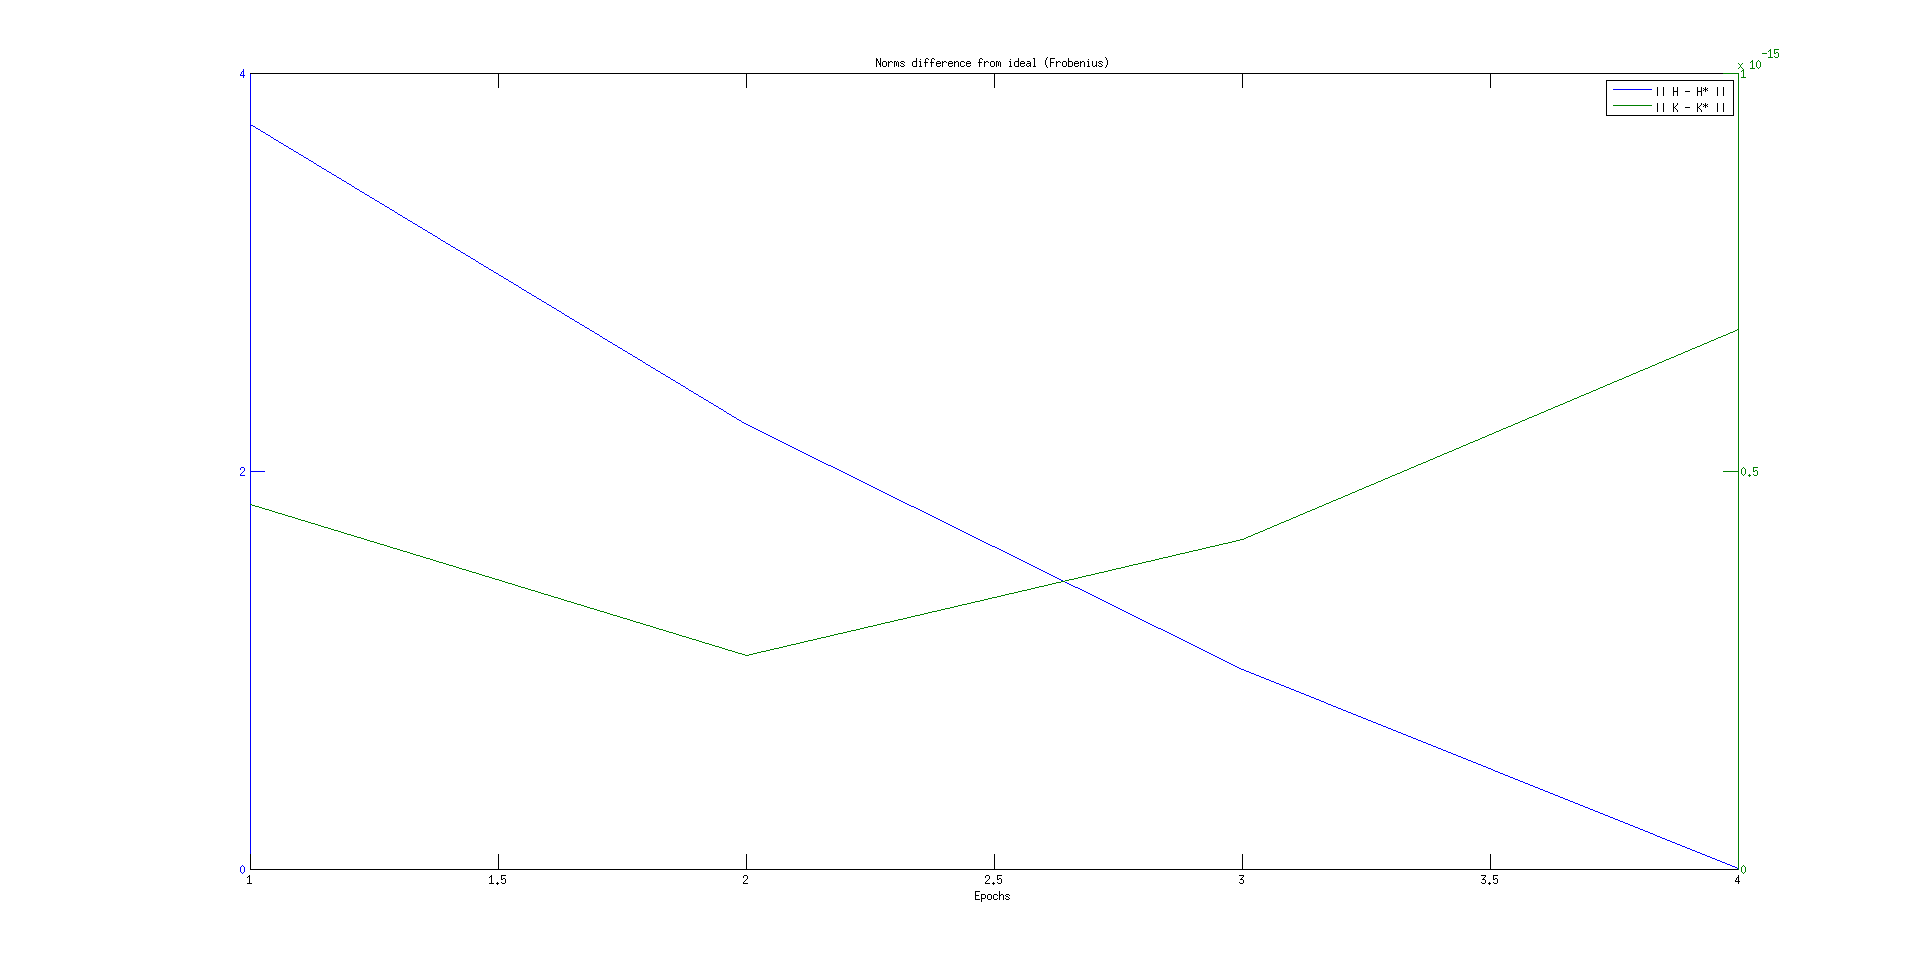
\includegraphics[scale=0.35]{norms.png}
\label{}
\end{figure}


Θεωρήσαμε αρχική συνθήκη $x_0 = (0.1, 0.1, 0.1)^T$. Οι αποκρίσεις σε κάθε εποχή φαίνονται παρακάτω.


\begin{figure}[H]
\centering
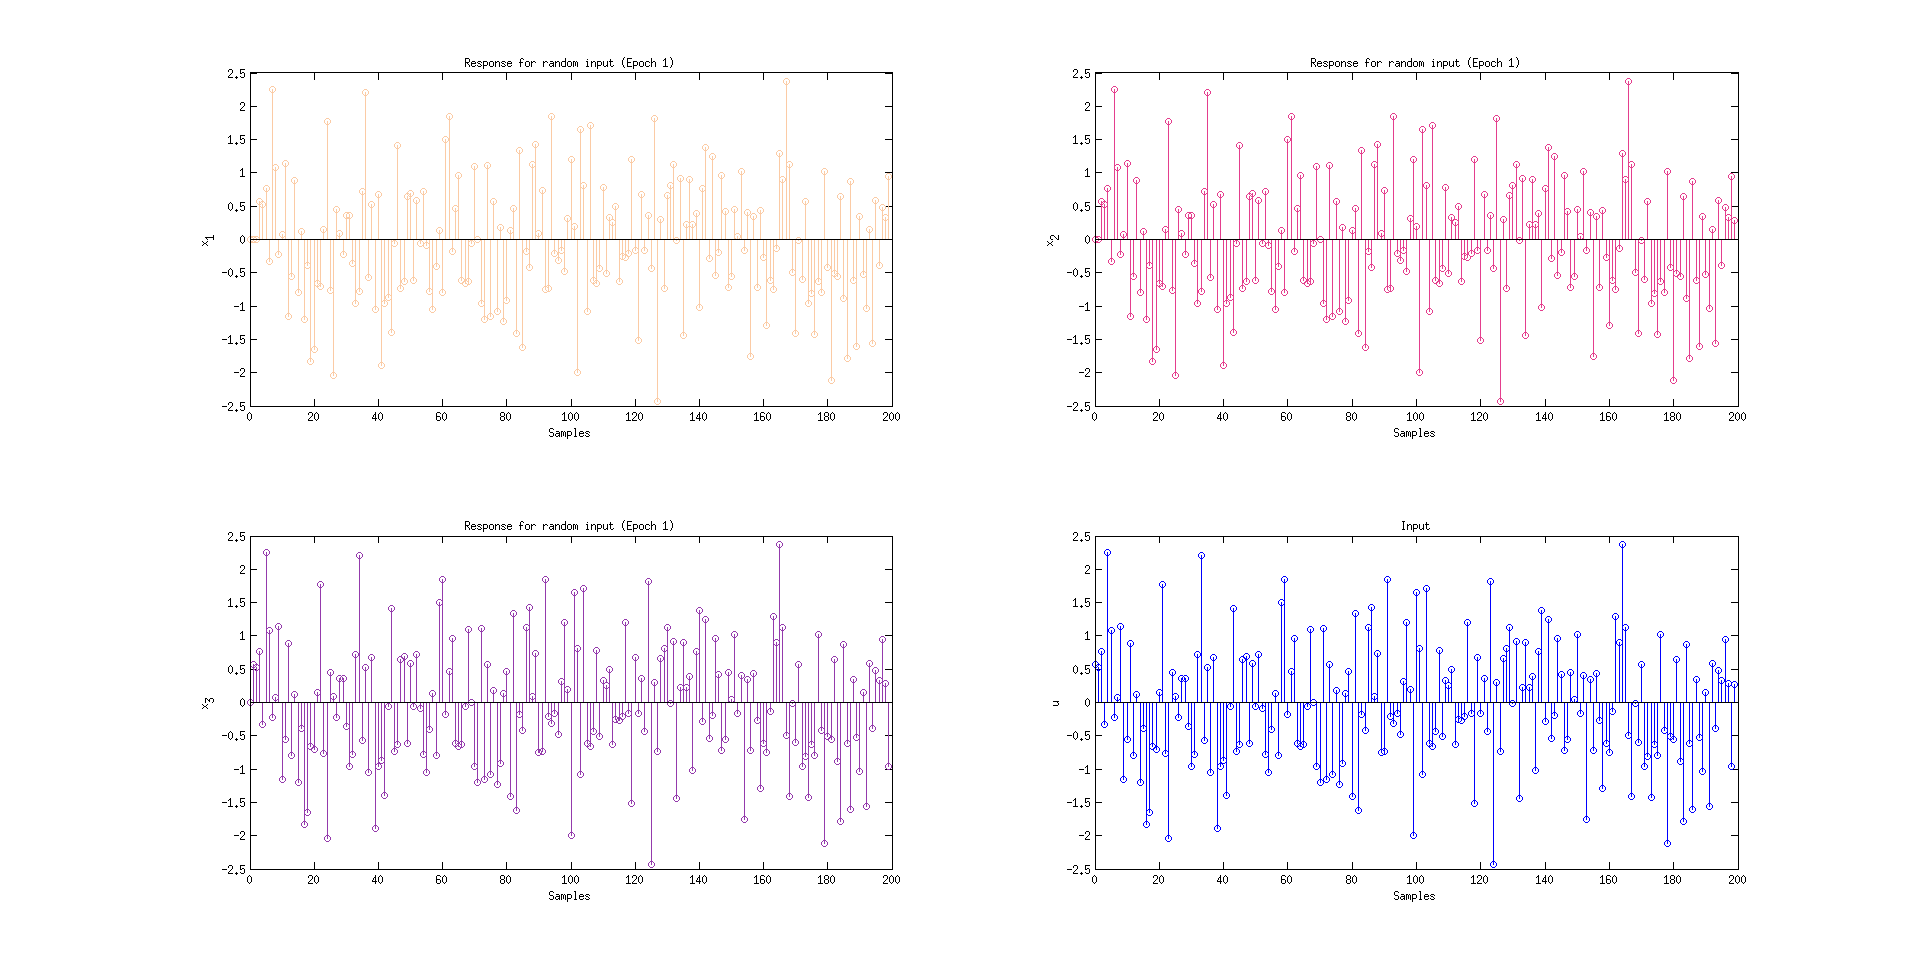
\includegraphics[scale=0.35]{s_1.png} \\
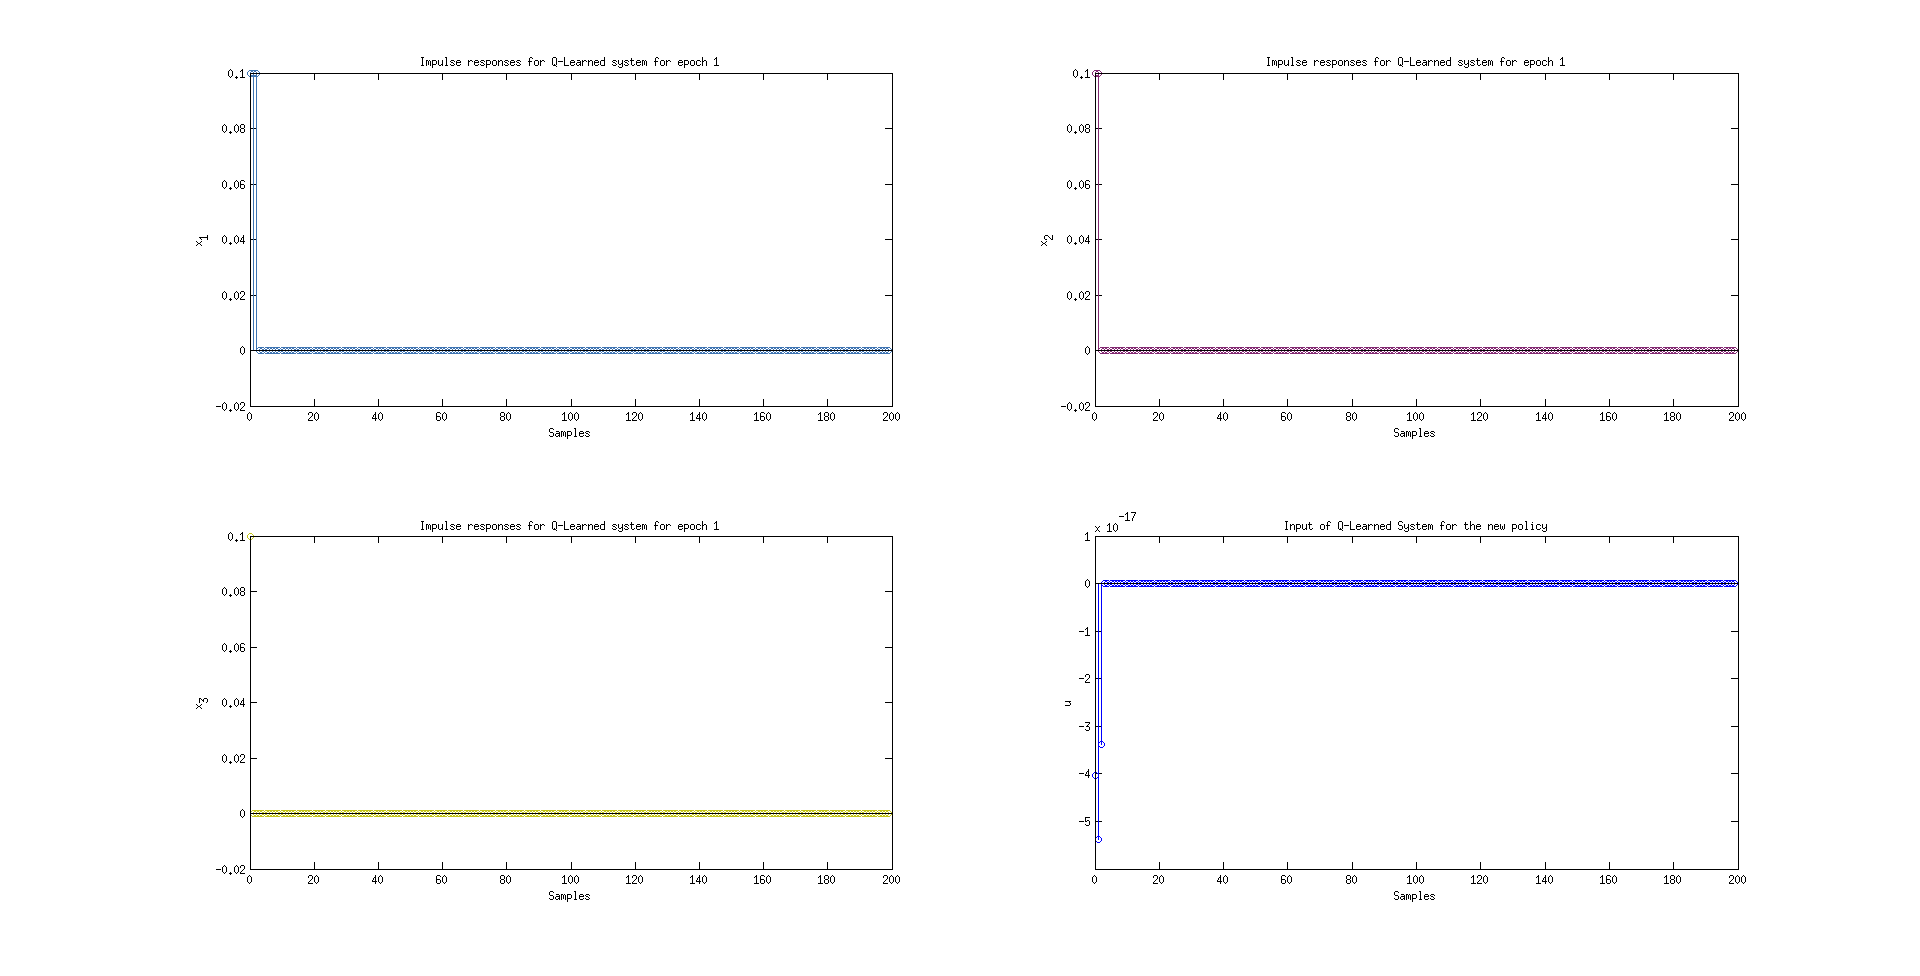
\includegraphics[scale=0.35]{q_1.png} \\
\label{}
\end{figure}

\begin{figure}[H]
\centering
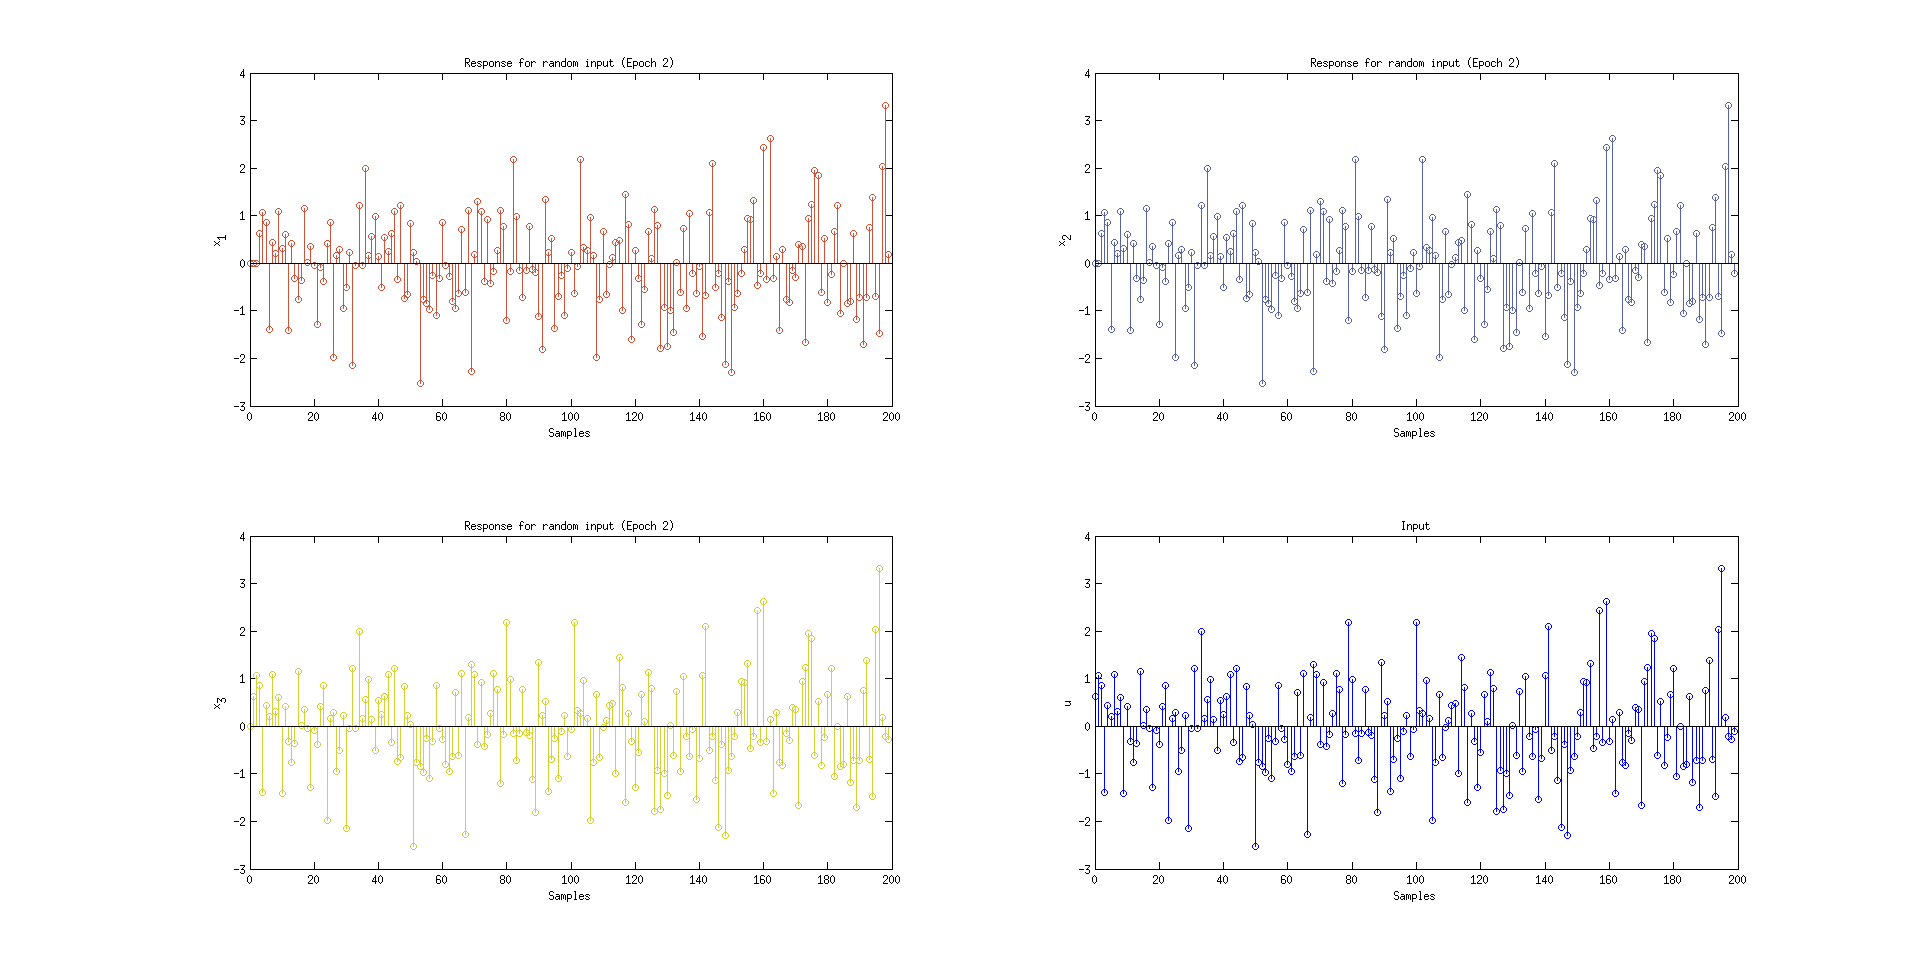
\includegraphics[scale=0.35]{s_2.png} \\
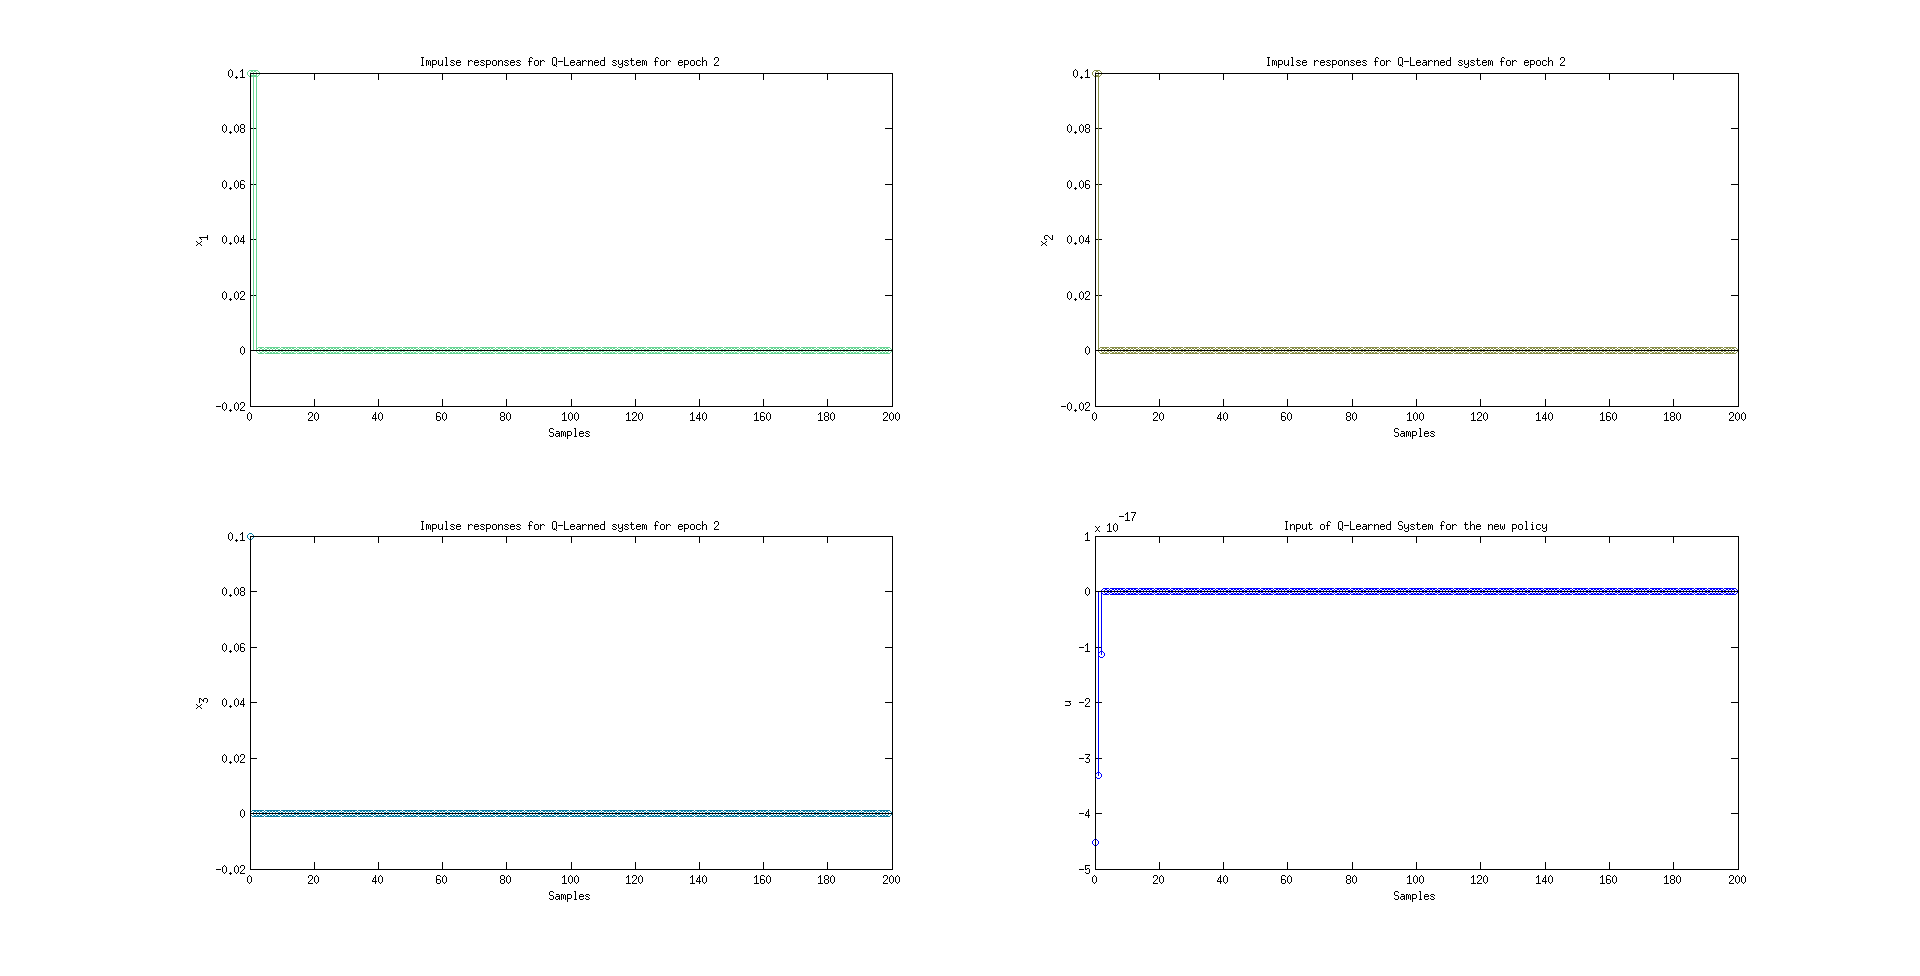
\includegraphics[scale=0.35]{q_2.png} \\
\label{}
\end{figure}

\begin{figure}[H]
\centering
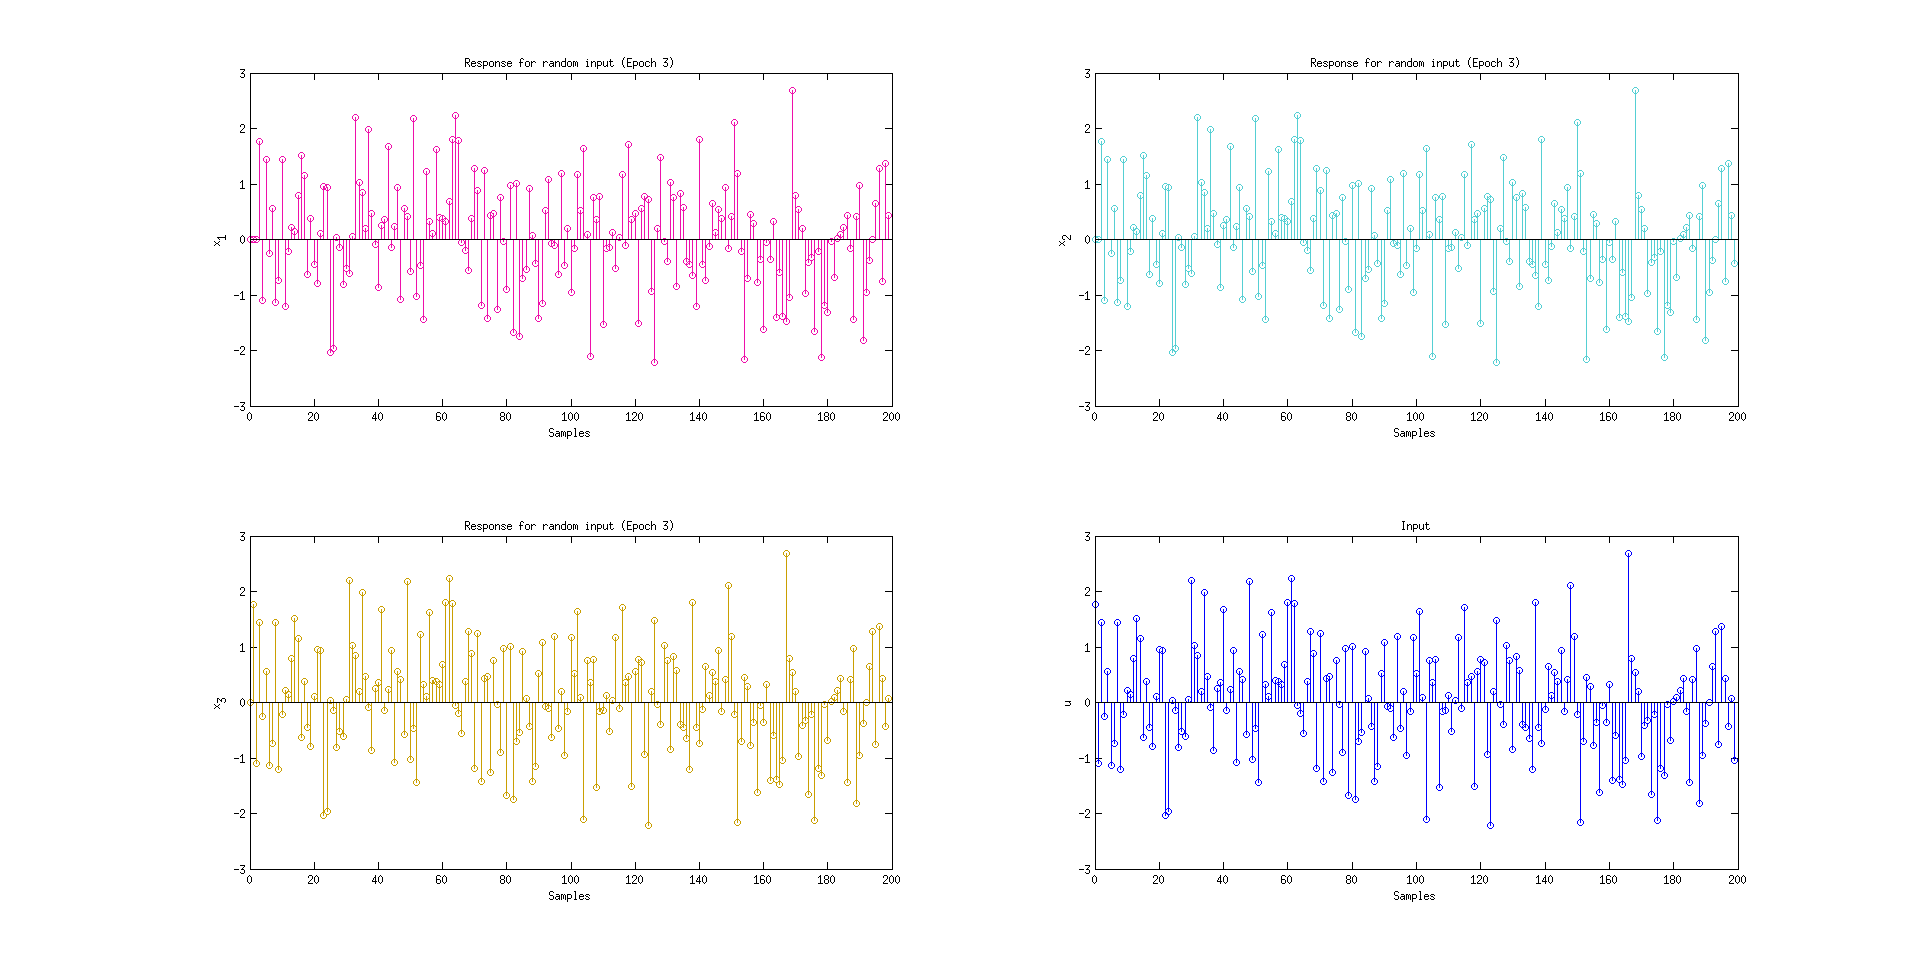
\includegraphics[scale=0.35]{s_3.png} \\
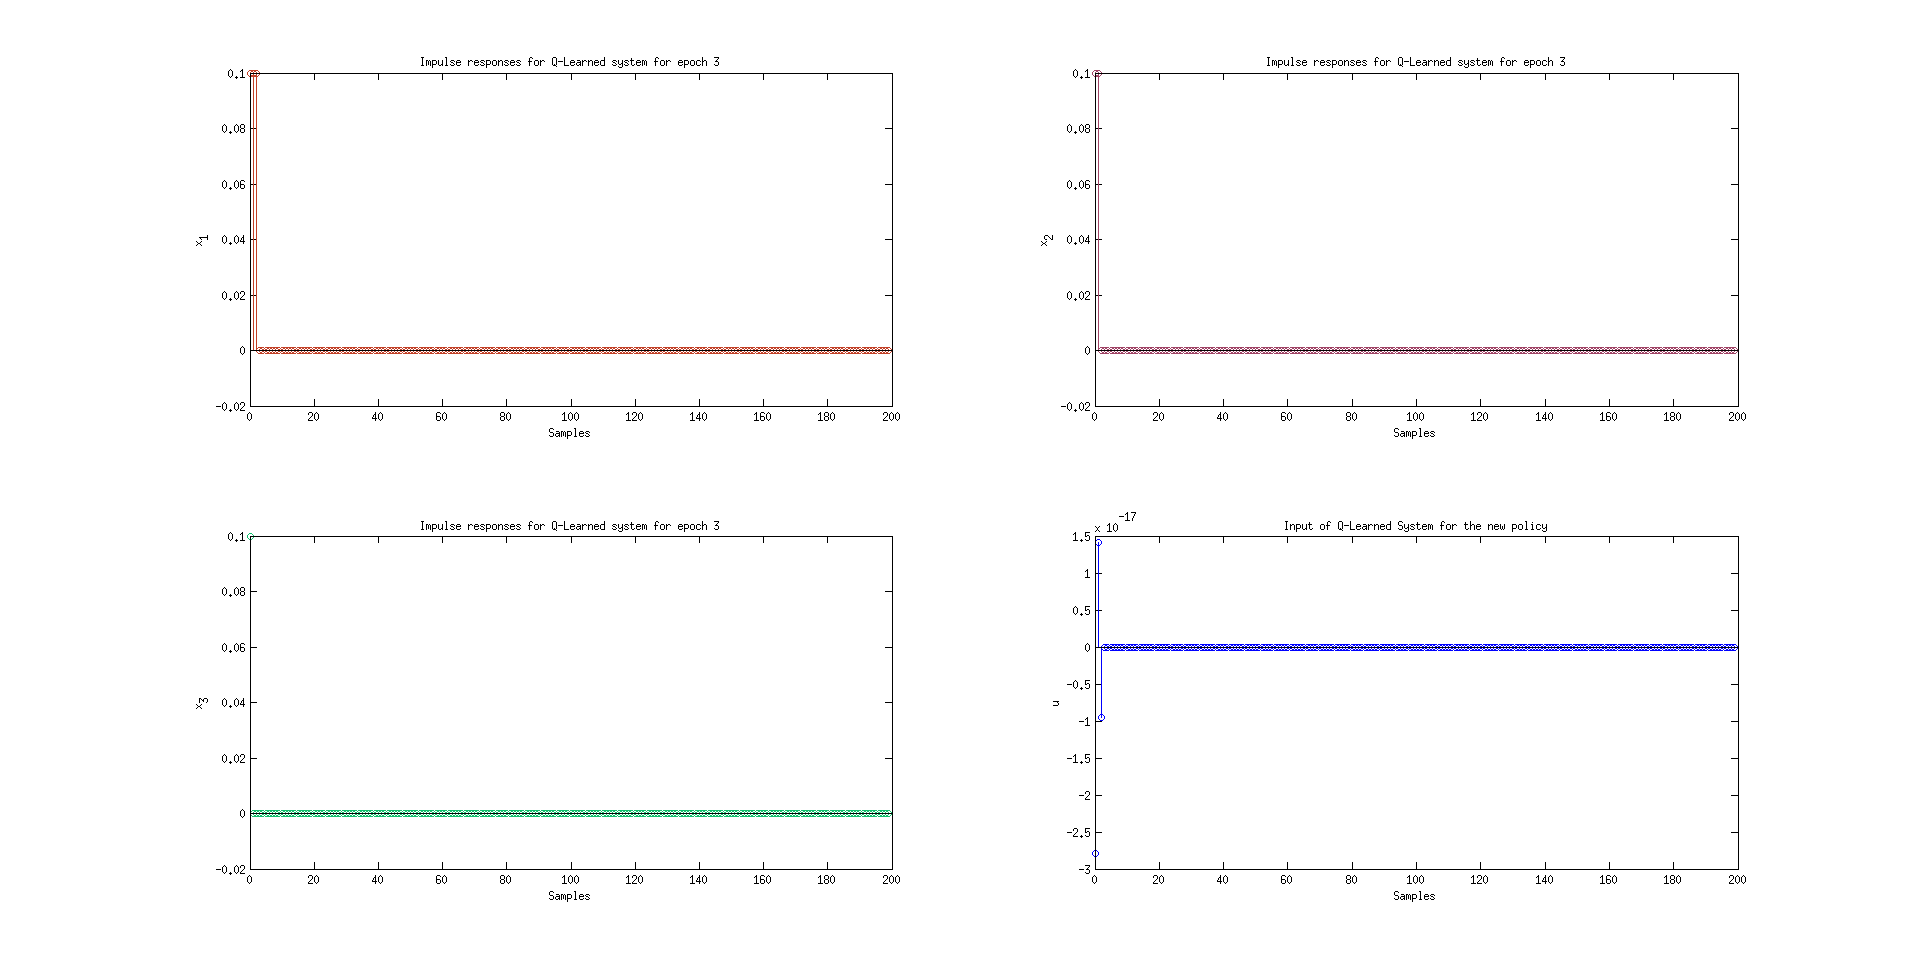
\includegraphics[scale=0.35]{q_3.png} \\
\label{}
\end{figure}

\begin{figure}[H]
\centering
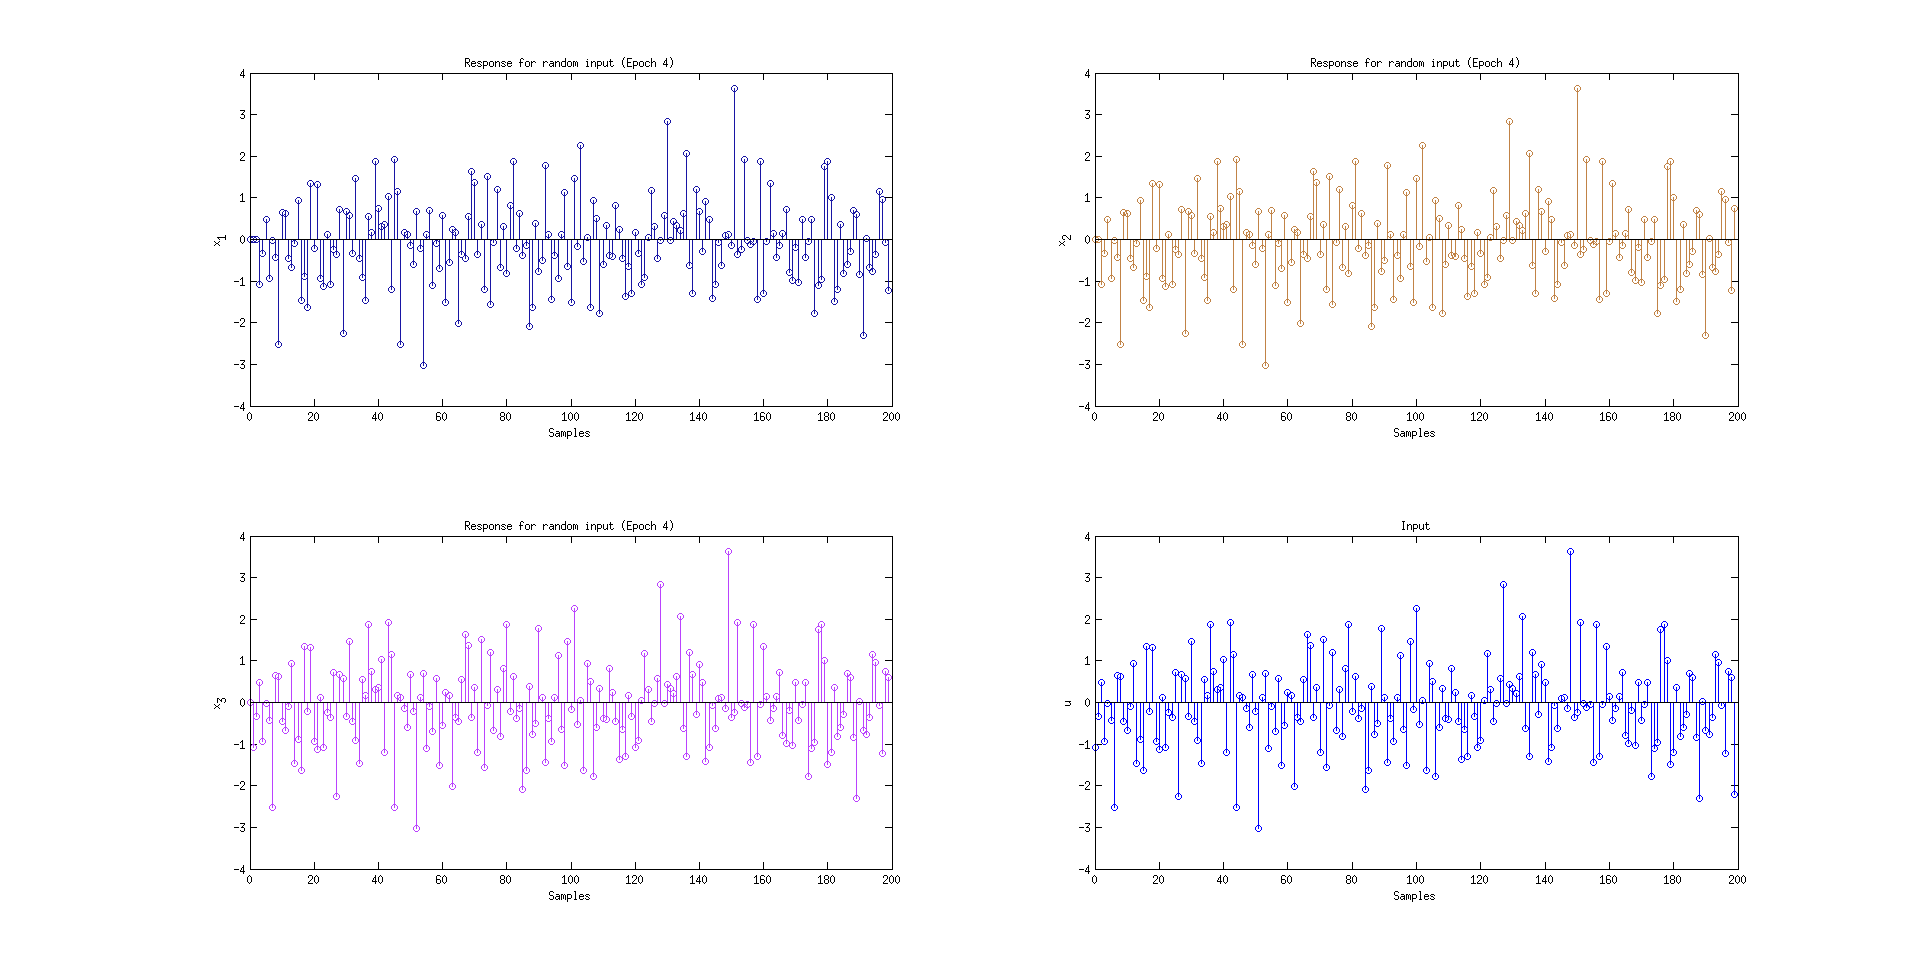
\includegraphics[scale=0.35]{s_4.png} \\
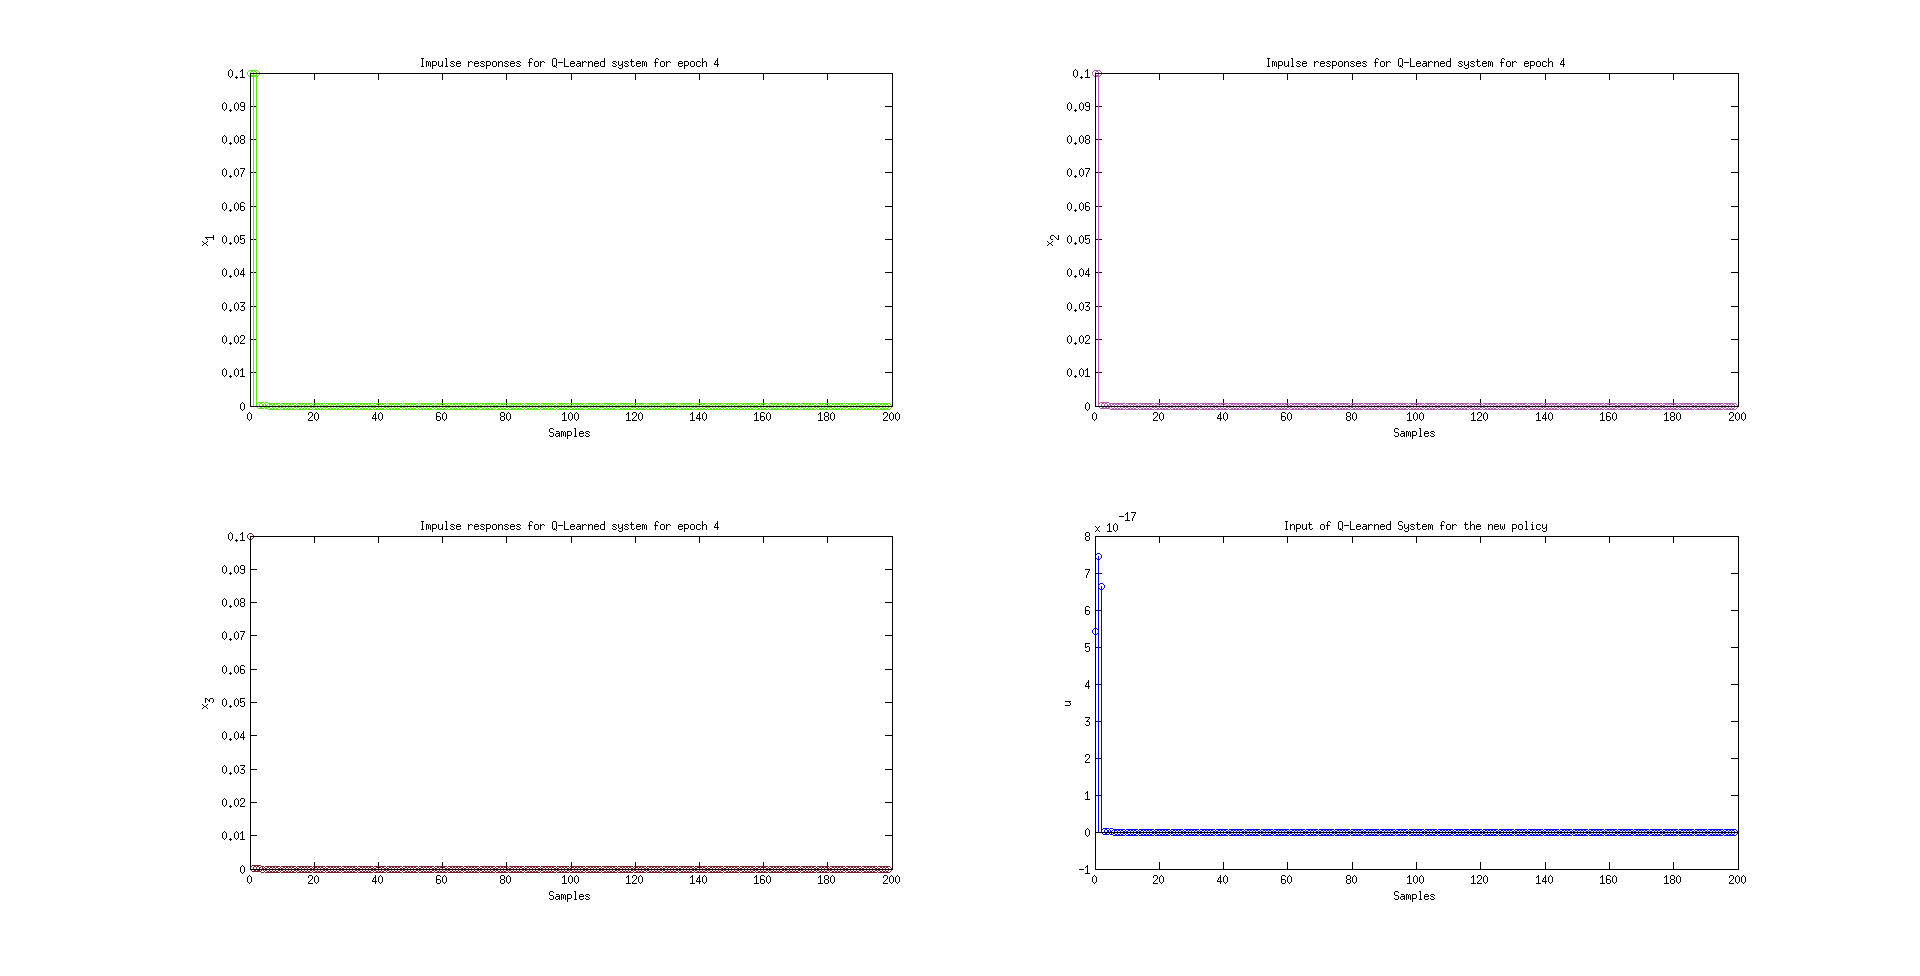
\includegraphics[scale=0.35]{q_4.png} \\
\label{}
\end{figure}


\section{Πηγαίος Κώδικας}


(Ζητούμενο Α) Για τον υπολογισμό των $H, K$ 

\lstinputlisting[language=matlab]{q_learning.m}


(Ζητούμενο Β) Το κύριο αρχείο \texttt{main.m}

\lstinputlisting[language=matlab]{main.m}



\begin{thebibliography}{9}

\bibitem{paper} Bradtke, Steven J. "Reinforcement learning applied to linear quadratic regulation." Advances in neural information processing systems. 1993.

\end{thebibliography}

\end{document}




